\documentclass{article}
\usepackage{amsmath}
\usepackage{amssymb}
\usepackage{graphicx}
\usepackage{float}
\usepackage{multirow}
\usepackage{verbatim}

\setlength{\parindent}{0em}
\setlength{\parskip}{1em}
\renewcommand{\arraystretch}{1.5}

\newcommand{\diff}{\mathop{}\!\mathrm{d}}
\newcommand{\prob}{\mathbb{P}}
\newcommand{\expect}{\mathbb{E}}

\title{Assignment 5}
\author{Joshua Hwang (44302650)}
\date{13 May}

\begin{document}
\maketitle

\section{Approximate $S_{100}$}
Using the Central Limit Theorem we can approximate $\prob(S_{100} > 600)$.
We first note $\prob(S_{100} > x) = 1 - \prob(S_{100} \leq x)$. The right
hand side is much easier to work with so we'll be focussing on
$\prob(S_{100} \leq x)$.
\begin{align*}
    \prob \left( \frac{S_{100} - 100\mu}{\sigma \sqrt{100}} \leq x \right)
    &= \prob \left( S_{100} \leq 10 \sigma x + 100\mu \right) \\
    &\approx \Phi(x) \\
\end{align*}

We know $\mu = \frac{363}{65} \approx 5.5846$ but we need to find $\sigma$.
We find this by computing $\expect (X - \expect X)^2$.
\begin{align*}
    \text{Var} X &= \int_x (x - \mu)^2 f(x) \diff x \\
    &= \frac{3}{52} \int_1^9 (x - \frac{363}{65})^2 \sqrt{x} \diff x \\
    &= \frac{3}{52} \int_1^9
    \left( x^2 - 2x\frac{363}{65} + \frac{131769}{4225} \right)
    \sqrt{x} \diff x \\
    &= \frac{3}{52} \int_1^9
    x^{2.5} - \frac{726}{65}x^{1.5} + x^{0.5}\frac{131769}{4225} \diff x \\
    &= \frac{3}{52} \left[
    \frac{2}{7}x^{3.5} - \frac{1452}{325}x^{2.5} + x^{1.5}\frac{87846}{4225}
    \right]_1^9 \\
    &= \frac{3}{52} 83.9807 && \text{To four decimal places} \\
    &= 4.8450 \\
    \sigma &= 2.2011
    && \text{Standard deviation is the square root of Variance}
\end{align*}

Now,
\begin{align*}
    \prob \left( \frac{S_{100} - 100\mu}{\sigma \sqrt{100}} \leq x \right)
    &= \prob \left( S_{100} \leq 10 \sigma x + 100\mu \right) \\
    &= \prob \left( S_{100} \leq 10 \times 2.2011 x + 100 \times 5.5846 \right) \\
    &= \prob \left( S_{100} \leq 22.011 x + 558.46 \right)
\end{align*}

We ensure the right hand side of our probability is 600.
\begin{align*}
    600 &= 22.011 x + 558.46 \\
    x &= 1.8872 \\
\end{align*}

Now we need to find our probability using the graph provided,
\begin{align*}
    \Phi(1.8872) &\approx 0.97
\end{align*}

Now we answer the actual question,
\begin{align*}
    \prob(S_{100} > x) &= 1 - \prob(S_{100} \leq x) \\
    &= 1 - 0.97 \\
    &= 0.03 \\
    &= 3.0 \times 10^{-2} \\
\end{align*}

We create a Python program to simulate 10000 $S_{100}$ as well.
\verbatiminput{q1.py}

This gave us
\begin{verbatim}
Approx answer 0.0319
\end{verbatim}

Which fits closely to our own result of 0.0319.

\section{Column vector}
\subsection{Write out using vectors}
$Z$ is a $3\times1$ column vector of standard normals.
\begin{align*}
    X &= \mu + BZ \\
    X
    &=
    \begin{bmatrix}
        0 \\ 1 \\ -1
    \end{bmatrix}
    +
    \begin{bmatrix}
        1 & 0 & 0 \\
        0 & 2 & 0 \\
        0 & 0 & \sqrt{2} \\
    \end{bmatrix}
    Z \\
\end{align*}

\subsection{What is the covariance matrix of $X$}
We can look at the following scenario as a multivariate normal distribution
and use the $B B^T$ but we will instead use the definition of covariance
(this is mainly because I'm not sure how far in the lectures we've gone
and don't want to use advanced knowledge).

The covariance matrix defined for the $(i,j)$ element is,
\begin{align*}
    \text{Cov}(X_i,X_j) & = \expect (X_i - \mu_i)(X_j - \mu_j) \\
\end{align*}

It is obvious that if $i = j$ we just have variance and the elements
$(i, j) = (j ,i)$. Since all $X_i$ are independent we know
$\expect X_i X_j = \expect X_i \expect X_j$ when $i \neq j$.

Thus for the elements in our covariance matrix we have,
\begin{align*}
    \text{Cov}(X_i,X_j) & = \expect X_i X_j - \expect X_i \expect X_j \\
    & = \expect X_i \expect X_j - \expect X_i \expect X_j \\
    & = 0 \\
\end{align*}

Thus our matrix is now,
\begin{align*}
    \begin{bmatrix}
        1 & 0 & 0 \\
        0 & 4 & 0 \\
        0 & 0 & 2 \\
    \end{bmatrix}
\end{align*}

\subsection{Expectation of $Y_1$}
Find the expectation of $Y_1 = X_1 + X_3$. We will make use of helpful
properties of expectation.
\begin{align*}
    \expect Y_1 &= \expect X_1 + \expect X_3 \\
    &= 0 + -1 \\
    \expect Y_1 &= -1 \\
\end{align*}

\subsection{Distribution of $Y_2$}
Find the distribution of $Y_2 = X_1 + X_2 - 2X_3$. We note that normal
distributions are all affine transformations of the standard normal. Thus,
\begin{align*}
    Y_2 &= X_1 + X_2 - 2X_3 \\
    &= N(0,1) + (1 + 2 N(0,1)) - 2(-1 + \sqrt{2} N(0,1)) \\
    &= 3 + (3 - 2\sqrt{2}) N(0,1) \\
    &= N(3, (3-2\sqrt{2})^2) \\
\end{align*}

Thus $Y_2$ has a normal distribution with $\mu = 3$
and $\sigma = 3 - 2\sqrt{2}$.

\subsection{Give joint distribution of $Y_1$ and $Y_2$}
We consider a column vector $Y = \begin{bmatrix} Y_1 \\ Y_2 \end{bmatrix}$.
From here we attempt to put $Y$ in context of standard normals.
\begin{align*}
    Y &= \begin{bmatrix} Y_1 \\ Y_2 \end{bmatrix} \\
    &= \begin{bmatrix} X_1 & +0 & +X_3 \\ X_1 & +X_2 & -2X_3 \end{bmatrix} \\
    &= \begin{bmatrix} 1 & 0 & 1 \\ 1 & 1 & -2 \end{bmatrix}
    \begin{bmatrix} X_1 \\ X_2 \\ X_3 \end{bmatrix} \\
    &= \begin{bmatrix} 1 & 0 & 1 \\ 1 & 1 & -2 \end{bmatrix}
    \left(
        \begin{bmatrix}
            0 \\ 1 \\ -1
        \end{bmatrix}
        +
        \begin{bmatrix}
            1 & 0 & 0 \\
            0 & 2 & 0 \\
            0 & 0 & \sqrt{2} \\
        \end{bmatrix}
        Z
    \right) \\
    &= \begin{bmatrix} 1 & 0 & 1 \\ 1 & 1 & -2 \end{bmatrix}
    \begin{bmatrix}
        0 \\ 1 \\ -1
    \end{bmatrix}
    +
    \begin{bmatrix} 1 & 0 & 1 \\ 1 & 1 & -2 \end{bmatrix}
    \begin{bmatrix}
        1 & 0 & 0 \\
        0 & 2 & 0 \\
        0 & 0 & \sqrt{2} \\
    \end{bmatrix}
    Z  \\
    &= \begin{bmatrix} -1 \\ 3 \end{bmatrix}
    +
    \begin{bmatrix}
        1 & 0 & \sqrt{2} \\
        1 & 2 & -2\sqrt{2} \\
    \end{bmatrix}
    Z
\end{align*}

From here we can calculate the covariance matrix $\Sigma = BB^T$ and obtain
the pdf for the joint distribution.
\begin{align*}
    \Sigma &= BB^T \\
    &=
    \begin{bmatrix}
        1 & 0 & \sqrt{2} \\
        1 & 2 & -2\sqrt{2} \\
    \end{bmatrix}
    \begin{bmatrix}
        1 & 1 \\
        0 & 2 \\
        \sqrt{2} & -2\sqrt{2}
    \end{bmatrix} \\
    &=
    \begin{bmatrix}
        3 & -3 \\
        -3 & 13
    \end{bmatrix}
\end{align*}

Note the determinant for $\Sigma \neq 0$ thus our matrix is invertible.
\begin{align*}
    \begin{bmatrix}
        3 & -3 \\
        -3 & 13
    \end{bmatrix}^{-1}
    &= \frac{1}{13 \times 3 - 3 \times 3}
    \begin{bmatrix}
        13 & 3 \\
        3 & 3
    \end{bmatrix} \\
    &= \frac{1}{30}
    \begin{bmatrix}
        13 & 3 \\
        3 & 3
    \end{bmatrix} \\
\end{align*}

We know substitute our values into the jointly normal pdf.
($n=2$ is the dimension of $Y$)
\begin{align*}
    f_Y(y) &= \frac{1}{\sqrt{(2\pi)^n det(\Sigma)}}
    e^{-\frac{1}{2} (y-\mu)^T \Sigma^{-1} (y-\mu)} \\
    &= \frac{1}{2\pi\sqrt{30}}
    e^{-\frac{1}{60} \left(y-\begin{bmatrix} -1 \\ 3 \end{bmatrix}\right)^T
    \begin{bmatrix}
        13 & 3 \\
        3 & 3
    \end{bmatrix} \left(y-\begin{bmatrix} -1 \\ 3 \end{bmatrix}\right)} \\
\end{align*}

\section{Comparing travel times}
\subsection{Compare expected travel times}
Each stage is independent of the others and is a basic sum. Thus we only have
to compute the sum of expected values from each stage.

For Albert,
\begin{align*}
    \mu_1 + \mu_2 + \mu_3 &= 5 + 12 + 20 \\
    &= 37 \text{minutes} \\
\end{align*}

For Bertha,
\begin{align*}
    \mu_1 + \mu_2 &= 15 + 20 \\
    &= 35 \text{minutes} \\
\end{align*}

\subsection{Probability that Albert arrives before Bertha}
We know both Albert's and Bertha's travel time can be modelled as a sum of
independent Normal distributions, which is in turn a normal distribution.

Proof that the sum of independent normal distributions is normal.
Consider $Y$ a sum of independent random normals.
We first note the moment generating function of $N(\mu,\sigma^2)$
\begin{align*}
    M_X(s) &= \expect e^{sX}
    &= e^{\mu s + \frac{1}{2} \sigma^2 s^2} \\
\end{align*}

We now try and calculate the moment generating function for $Y$.
\begin{align*}
    M_Y(s) &= \expect \left(e^{s\left(a + \sum_{i=1}^n b_i X_i\right)}\right) \\
    &= \expect \left(e^{s\left(a + \sum_{i=1}^n b_i X_i\right)}\right) \\
    &= e^{as} \prod_{i=1}^n \expect e^{s b_i X_i} \\
    &= e^{as} \prod_{i=1}^n M_{X_i} (s b_i) \\
    &= e^{as} \prod_{i=1}^n e^{\mu_i (s b_i) + \frac{1}{2} \sigma_i^2 (s b_i)^2} \\
    &= e^{as + s \sum_{i=1}^n \mu_i b_i + \frac{1}{2} \sigma_i^2 s^2 b_i^2} \\
\end{align*}

Which we can see is the moment generating function of a normal distribution.
With $\mu = a + \sum_{i=1}^n b_i \mu_i$
and $\sigma^2 = \sum_{i=1}^n b_i^2 \sigma_i^2$

For Albert,
\begin{align*}
    A &\sim N(5,1) + N(12,9) + N(20,16) \\
    A &\sim N(37, 26)
\end{align*}

For Bertha,
\begin{align*}
    B &\sim N(15, 4) + N(20, 3) \\
    B &\sim N(35, 7) \\
\end{align*}

Instead of determining when $\prob (A < B)$ we look at $\prob (A - B < 0)$.
This can be done easily since $A - B$ will be a normal distribution.

For $A - B$,
\begin{align*}
    A - B &\sim N(37, 26) - N(35, 7) \\
    A - B &\sim N(2, 19) \\
\end{align*}

Now we find,
\begin{align*}
    \prob(A-B<0) &= \prob\left(\frac{(A-B)-2}{\sqrt{19}}<\frac{-2}{\sqrt{19}}\right) \\
    &= \Phi\left(\frac{-2}{\sqrt{19}}\right)
\end{align*}

\section{An interesting moment generating function}
\begin{align*}
    M(t) &= \frac{1}{2} e^{\frac{t^2}{4}} (t^2+2)
\end{align*}

\subsection{Find $Var(X_i)$}
The moment generating function allows us to set $\expect X^n = M^(n)(0)$.
Thus we can get $Var(X) = M''(0) - (M'(0))^2$.
\begin{align*}
    M(t) &= \frac{1}{2} e^{\frac{t^2}{4}} (t^2+2) \\
    M'(t) &= \frac{t}{4} e^{\frac{t^2}{4}} (t^2+2)
    + t e^{\frac{t^2}{4}} \\
    M'(t) &= \frac{1}{4} t \left(t^2+6\right) e^{\frac{t^2}{4}} \\
    M''(t) &= \frac{1}{4} \left(t^2+6\right) e^{\frac{t^2}{4}}
    + \frac{1}{4} 2t^2 e^{\frac{t^2}{4}}
    + \frac{1}{8} t^2 \left(t^2+6\right) e^{\frac{t^2}{4}} \\
    M''(t) &= \frac{1}{8} \left(t^4 + 12t^2 + 12\right) e^{\frac{t^2}{4}} \\
\end{align*}

Since all $X_i$ are iid, the following Variance applies for all $X_i$.
\begin{align*}
    Var(X_i) &= M''(0) - (M'(0))^2 \\
    &= \frac{1}{8} \left(0^4 + 12(0)^2 + 12\right) e^{\frac{0^2}{4}}
    - \left(\frac{1}{4} (0) \left(0^2+6\right) e^{\frac{0^2}{4}}\right)^2 \\
    &= \frac{12}{8} \\
    &= \frac{3}{2} \\
\end{align*}

\subsection{Find MGF $\frac{S_n}{\sqrt{3n/2}}$}
Since $S_n = \sum_{i=1}^n X_i$ we can substitute into the definition of MGF.
\begin{align*}
    M_{\frac{S_n}{\sqrt{3n/2}}}(s) &= \expect e^{s \frac{S_n}{\sqrt{3n/2}}} \\
    &= \expect e^{S_n \frac{s}{\sqrt{3n/2}}} \\
    &= \prod_{i=1}^n \expect e^{X_i \frac{s}{\sqrt{3n/2}}} && \text{Since $S_n$ is a sum of iids} \\
    &= \prod_{i=1}^n M_{X_i} \left(\frac{s}{\sqrt{3n/2}}\right) \\
    &= M_{X_i} \left(\frac{s}{\sqrt{3n/2}}\right)^n && \text{Same MGF for all $i$} \\
    &= \left(\frac{1}{2} e^{\frac{\left(\frac{s}{\sqrt{3n/2}}\right)^2}{4}}
    \left(\left(\frac{s}{\sqrt{3n/2}}\right)^2+2\right)\right)^n \\
    &= \left(\frac{1}{2} e^{\frac{2s^2}{12n}} \left(\frac{2s^2}{3n}+2\right)\right)^n \\
    &= frac{1}{2^n} e^{\frac{s^2}{6}} (\frac{2s^2}{3n}+2)^n \\
    &= frac{1}{2^n} e^{\frac{s^2}{6}} 2^n (\frac{s^2}{3n}+1)^n \\
    &= e^{\frac{s^2}{6}} (\frac{\frac{s^2}{3}}{n}+1)^n \\
\end{align*}

Thus the MGF of $M_{\frac{S_n}{\sqrt{3n/2}}}(s) = e^{\frac{s^2}{6}} (\frac{\frac{s^2}{3}}{n}+1)^n$.

\subsection{Find what happens when $n \to \infty$}
We first note
\begin{align*}
    \lim_{n \to \infty} (\frac{x}{n} + 1)^n &= e^x
\end{align*}

Thus
\begin{align*}
    M_{\frac{S_n}{\sqrt{3n/2}}}(s)
    &= e^{\frac{s^2}{6}} (\frac{\frac{s^2}{3}}{n}+1)^n \\
    &= e^{\frac{s^2}{6}} e^{\frac{s^2}{3}}\\
    &= e^{\frac{s^2}{2}} \\
\end{align*}

\section{Consider random variable $X+Y$}
Since $X$ and $Y$ are independent the joint pdf for $X+Y$ is,
\begin{align*}
    f(x,y) &= f_X(x) f_Y(y) \\
    &= \frac{1}{1} e^{-y} && x \in [0,1] \\
    &= e^{-y} && x \in [0,1] \\
\end{align*}

\subsection{Compute $\prob(X+Y>z)$}
We note,
\begin{align*}
    \prob(X+Y>z) &= 1 - \prob(X+Y \leq Z)
\end{align*}

and,
\begin{align*}
    X + Y &\leq z \\
    Y &\leq z - X \\
\end{align*}

We now use our pdf to integrate over all values that satisfy $Y \leq z - X$.
\begin{align*}
    \prob(X+Y \leq z) &= \iint_{Y \leq z - X} e^{-y} \diff y \diff x
\end{align*}

We now have two cases, when $0 \leq z \leq 1$ and $z > 1$.
We first explore the $0 \leq z \leq 1$ case,
\begin{align*}
    \iint_{Y \leq z - X} e^{-y} \diff y \diff x
    &= \int_0^z \int_0^{-x+z} e^{-y} \diff y \diff x \\
    &= \int_0^z - \left[ e^{-y} \right]_0^{-x+z} \diff x \\
    &= \int_0^z 1 - e^{x} e^{-z} \diff x \\
    &= \left[ x - e^{x} e^{-z} \right]_0^z \\
    &= z + e^{-z} - 1 \\
\end{align*}

Which we use to find, $\prob(X+Y>z) = 1 - \prob(X+Y \leq Z)$.
\begin{align*}
    \prob(X+Y>z) &= 1 - \prob(X+Y \leq Z) \\
    &= 1 - (z + e^{-z} - 1) \\
    &= 2 - z - e^{-z}
\end{align*}

Now consider $z > 1$.
\begin{align*}
    \iint_{Y \leq z - X} e^{-y} \diff y \diff x
    &= \int_0^1 \int_0^{-x+z} e^{-y} \diff y \diff x \\
    &= \int_0^1 - \left[ e^{-y} \right]_0^{z-x}  \diff x \\
    &= \int_0^1 1 - e^{-(z-x)} \diff x \\
    &= \int_0^1 1 - e^{x-z} \diff x \\
    &= \int_0^1 1 - e^{x} e^{-z} \diff x \\
    &= \left[ x - e^{x} e^{-z} \right]_0^1 \\
    &= 1 - e^{1-z} + e^{-z} \\
    &= 1 + (1 - e)e^{-z} \\
\end{align*}

Which we use to find, $\prob(X+Y>z) = 1 - \prob(X+Y \leq Z)$.
\begin{align*}
    \prob(X+Y>z) &= 1 - \prob(X+Y \leq Z) \\
    &= 1 - (1 + (1 - e)e^{-z}) \\
    &= -(1 - e)e^{-z} \\
    &= (e - 1)e^{-z}
\end{align*}

Thus $\prob(X+Y>z)$ will be determined by $2 - z - e^{-z}$ when
$0 \leq z \leq 1$ and $(e - 1)e^{-z}$ when $z > 1$.

\subsection{Plot $X+Y$}
To make this easier to understand we will consider $Z=X+Y$.
From the previous section we have $\prob(Z \leq z)$ as a piecewise function.
\begin{align*}
    \prob(Z \leq z)
    &=
    \begin{cases}
        z + e^{-z} - 1 & 0 \leq z \leq 1 \\
        1 + (1 - e)e^{-z} & z > 1 \\
    \end{cases}
\end{align*}

To get the pdf we must differentiate the above function. This is fine since
our function is continuous for all points (observe $z=1$ is equal for both
sides of the piecewise).
\begin{align*}
    \prob(Z \leq z) = F(z)
    &=
    \begin{cases}
        z + e^{-z} - 1 & 0 \leq z \leq 1 \\
        1 + (1 - e)e^{-z} & z > 1 \\
    \end{cases} \\
    f(z) &=
    \begin{cases}
        1 - e^{-z} & 0 \leq z \leq 1 \\
        - (1 - e)e^{-z} & z > 1 \\
    \end{cases} \\
    &=
    \begin{cases}
        1 - e^{-z} & 0 \leq z \leq 1 \\
        (e - 1)e^{-z} & z > 1 \\
    \end{cases} \\
\end{align*}

This piecewise function is graphed below,
\begin{figure}[H]
    \centering
    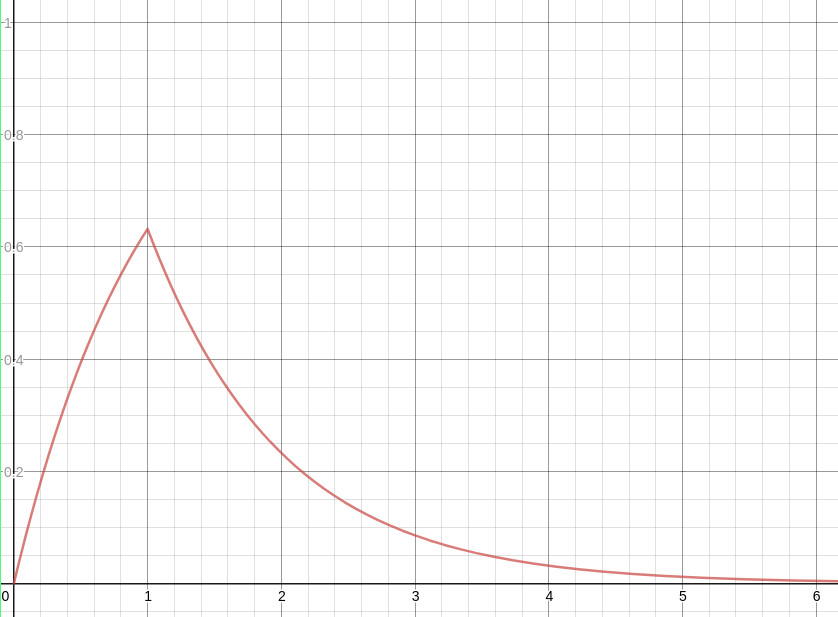
\includegraphics[width=5in]{graph.jpg}
\end{figure}

\subsection{Find MGF of $X+Y$}
MGF is defined by,
\begin{align*}
    M(s) &= \expect e^{sZ} \\
    &= \int_0^\infty f(z) e^{sz} \diff z \\
    &= \int_0^1 f(z) e^{sz} \diff z + \int_1^\infty f(z) e^{sz} \diff z \\
    &= \int_0^1 (1 - e^{-z}) e^{sz} \diff z
    + \int_1^\infty (e - 1) e^{-z} e^{sz} \diff z \\
    &= \int_0^1 e^{sz} - e^{z(s-1)} \diff z
    + \int_1^\infty (e - 1) e^{(s-1)z} \diff z \\
    &= \left[ \frac{1}{s} e^{sz} - \frac{1}{s-1} e^{z(s-1)} \right]_0^1
    + \left[ \frac{e - 1}{s - 1} e^{(s-1)z} \right]_1^\infty \\
    &= \frac{1}{s} e^{s} - \frac{1}{s-1} e^{s-1} - \left( \frac{1}{s} - \frac{1}{s-1} \right)
    - \frac{e - 1}{s - 1} e^{s-1} \\
    \text{Only when $s < 1$} \\
    &= \frac{e^{s}}{s} - \frac{e^{s-1}}{s-1} - \frac{1}{s} + \frac{1}{s-1}
    - \frac{e^{s} - e^{s-1}}{s - 1} \\
    &= \frac{e^{s}-1}{s} + \frac{1 - e^{s-1} - e^{s} + e^{s-1}}{s-1} \\
    &= \frac{e^{s}-1}{s} + \frac{1 - e^{s}}{s-1} \\
    &= \frac{1 - e^{s}}{s(s - 1)}
\end{align*}

Thus the MGF for $X + Y$ will be $M(s) = \frac{1 - e^{s}}{s(s - 1)}$
only when $s < 1$.

\end{document}
